In this problem, we are going to learn the class of $k$-decision
lists. A decision list is an ordered sequence of if-then-else
statements. The sequence of if-then-else conditions are tested in
order, and the answer associated to the first satisfied condition is
output. See Figure~\ref{fig:decision_list} for an example of a
$2$-decision list.

\begin{figure}[!h]
\begin{center}
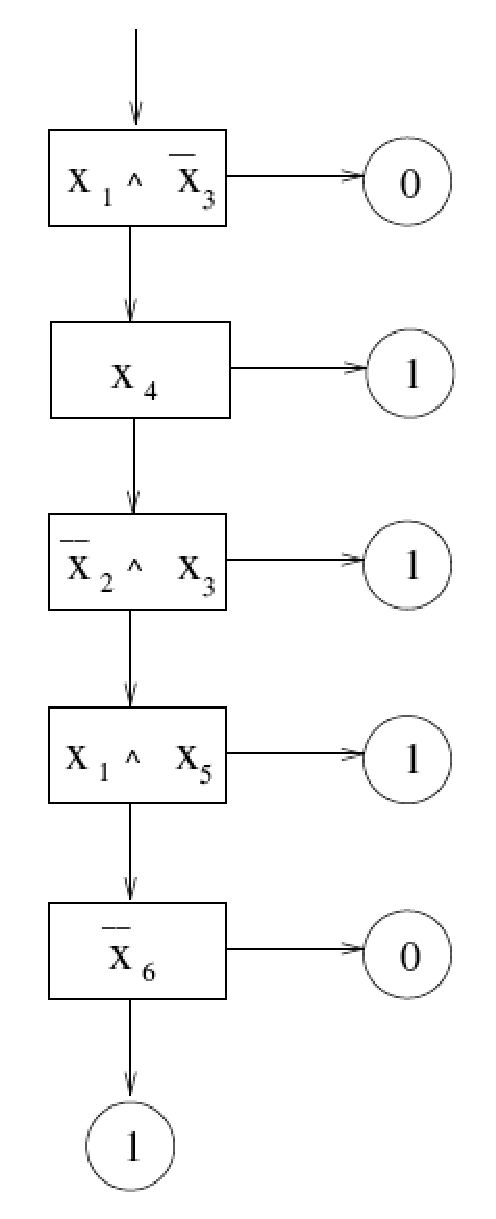
\includegraphics[width=1.35in]{fig-1.pdf}
\caption{A $2$-decision list.}
\label{fig:decision_list}
\end{center}
\end{figure}

A {\em $k$-decision list} over the variables $x_{1}, \ldots, x_{n}$ is
an ordered sequence $L=(c_{1}, b_{1}), \ldots, (c_{\ell},b_{\ell})$ and a
bit $b$, in which each $c_{i}$ is a conjunction of at most $k$
literals over $x_{1},\ldots, x_{n}$. The bit $b$ is called the {\em
  default} value, and $b_{i}$ is referred to as the bit {\em
  associated} with condition $c_{i}$. For any input $x \in \{0,
1\}^{n}$, $L(x)$ is defined to be the bit $b_{j}$, where $j$ is the
smallest index satisfying $c_{j}(x)=1$; if no such index exists, then
$L(x)=b$.

We denote by $k\mbox{\em -DL}$ the class of concepts that can be
represented by a $k$-decision list.


\begin{enumerate}
\item \relax[8 points] Show that if a concept $c$ can be represented
  as a $k$-decision list so can its complement, $\neg c$. You can show
  this by providing a $k$-decision list that represents $\neg c$,
  given $c = \{(c_{1},b_{1}), \ldots, (c_{\ell},b_{\ell}),b\}$.

\begin{itemize}
\item To prove that the complement of $c$ is a $k$-decision list, we can simply take $c$ and negate all of the bits to produce another $k$-decision list. It would look such as the following: $\neg c = \{(c_{1},\neg b_{1}), \ldots, (c_{\ell},\neg b_{\ell}),\neg b\}$, which is a $k$-decision list.
\end{itemize}
\item \relax[9 points] Use  Occam's Razor to show: \\
  For any constant $k \geq 1$, the class of $k$-decision lists is
  PAC-learnable.

\begin{itemize}
\item Occam's Razor states that the least complicated case is most likely true, but in this course we take it as being true. Therefore, we can show this to be PAC-learnable by finding a lower bound on the set such that it is the minimum $k$-decision list. This can be done by showing that the dimensions of data needed is {\em finite}.

It can be trivially seen that the size of the concept class is $\left| c_{k} \right| = \mathcal{O}\left( n^{k}\right)$. Each of the bits belong in $b_{i}\in \{ 0,1 \}$, and since there are $\ell$ of them it results in $2^{\ell}$ different combinations. There are also $\ell!$ orderings of those bits. Finally, the size of the concept class that can describe the data is $2^{\left| c_{k} \right|}$. Therefore, the overall bound is represented by the product of these three which is $\mathcal{O}\left( 2^{\left| c_{k} \right|}\cdot \ell!\cdot 2^{\ell} \right)$. However, the {\em maximum value} of $\ell$ is represented by $\left| c_{k} \right|$, so we can simplify our notation as $\mathcal{O}\left( 2^{2\left| c_{k}\right|}\left| c_{k} \right|!\right)$.

Finally, the size of the number of examples needed in our set is logarithmically proportional to the size of the concept class, so by taking the log we get $\mathcal{O}\left( 2n^{k}\log(2) + kn^{k}\log(n)\right)$ which is a {\em finite number} for any $k\geq 1$ and thus is PAC-learnable.
\end{itemize}
\item \relax[8 points] Show that $1$-decision lists are a linearly
  separable functions. (Hint: Find a weight vector that will make the
  same predictions a given $1$-decision list.)

\begin{itemize}
\item To do this, we need to construct our $\mathbf{x}$ vector and then our $\mathbf{w}$ vector where $\mathbf{w}$ is the weight vector defined as $\mathbf{w} = (\theta , w_{1}, w_{2}, \ldots , w_{\ell})^{T}$ with $\theta$ being the bias. We can define our $\mathbf{x}$ vector as $\mathbf{x} = (1, x_{1}, x_{2}, \ldots, x_{\ell})^{T}$ with the leading term being needed to support the bias. $x_{i}$ can be defined by the value of $b_{i}$, where $x_{i} = -1$ for $b_{i} = 0$, and $x_{i} = 1$ for $b_{i} = 1$. From here, we can create a threshold function to ``learn'' the $k$-decision list, which is defined as $\mathbf{w}^{T}\cdot \mathbf{x} \geq 0$.

In building $\mathbf{w}$, we can define each element of $w_{i} = b_{i}\cdot 2^{\ell+1-i}$ as to separate the individual data points. This would make the first few elements $\mathcal{O}\left(\pm 2^{\ell}\right)$ and the last elements $\mathcal{O}(\pm 2)$, where the $\pm$ comes about due to the individual bit $b_{i}$. Following this, we can look at the original 1-DL and if the overall/default bit is false, then we can set $\theta = -1$, else $\theta = 1$. This would overall be equivalent to the 1-DL and would make it liearly separable and learnable.
\end{itemize}
\end{enumerate}



%%% Local Variables: 
%%% mode: latex
%%% TeX-master: "hw3"
%%% End: 
